\documentclass{article}
\usepackage{graphicx}

% Language setting
% Replace `english' with e.g. `spanish' to change the document language
\usepackage[english]{babel}

% Set page size and margins
% Replace `letterpaper' with `a4paper' for UK/EU standard size
\usepackage[letterpaper,top=2cm,bottom=2cm,left=3cm,right=3cm,marginparwidth=1.75cm]{geometry}

\title{Problem Set 6}
\author{Trevor Jones}


\begin{document}
\maketitle

\section{Questions}
\begin{enumerate}
    \item Include in your .tex file an explanation of what the images are communicating. How
are they helpful for understanding your data set?
    \begin{enumerate}
        \item In the dataset I created, I am looking at Combine measurements and Quarterback Career performances in the NFL. 
    \end{enumerate}
\end{enumerate}

\begin{figure}
    \centering
    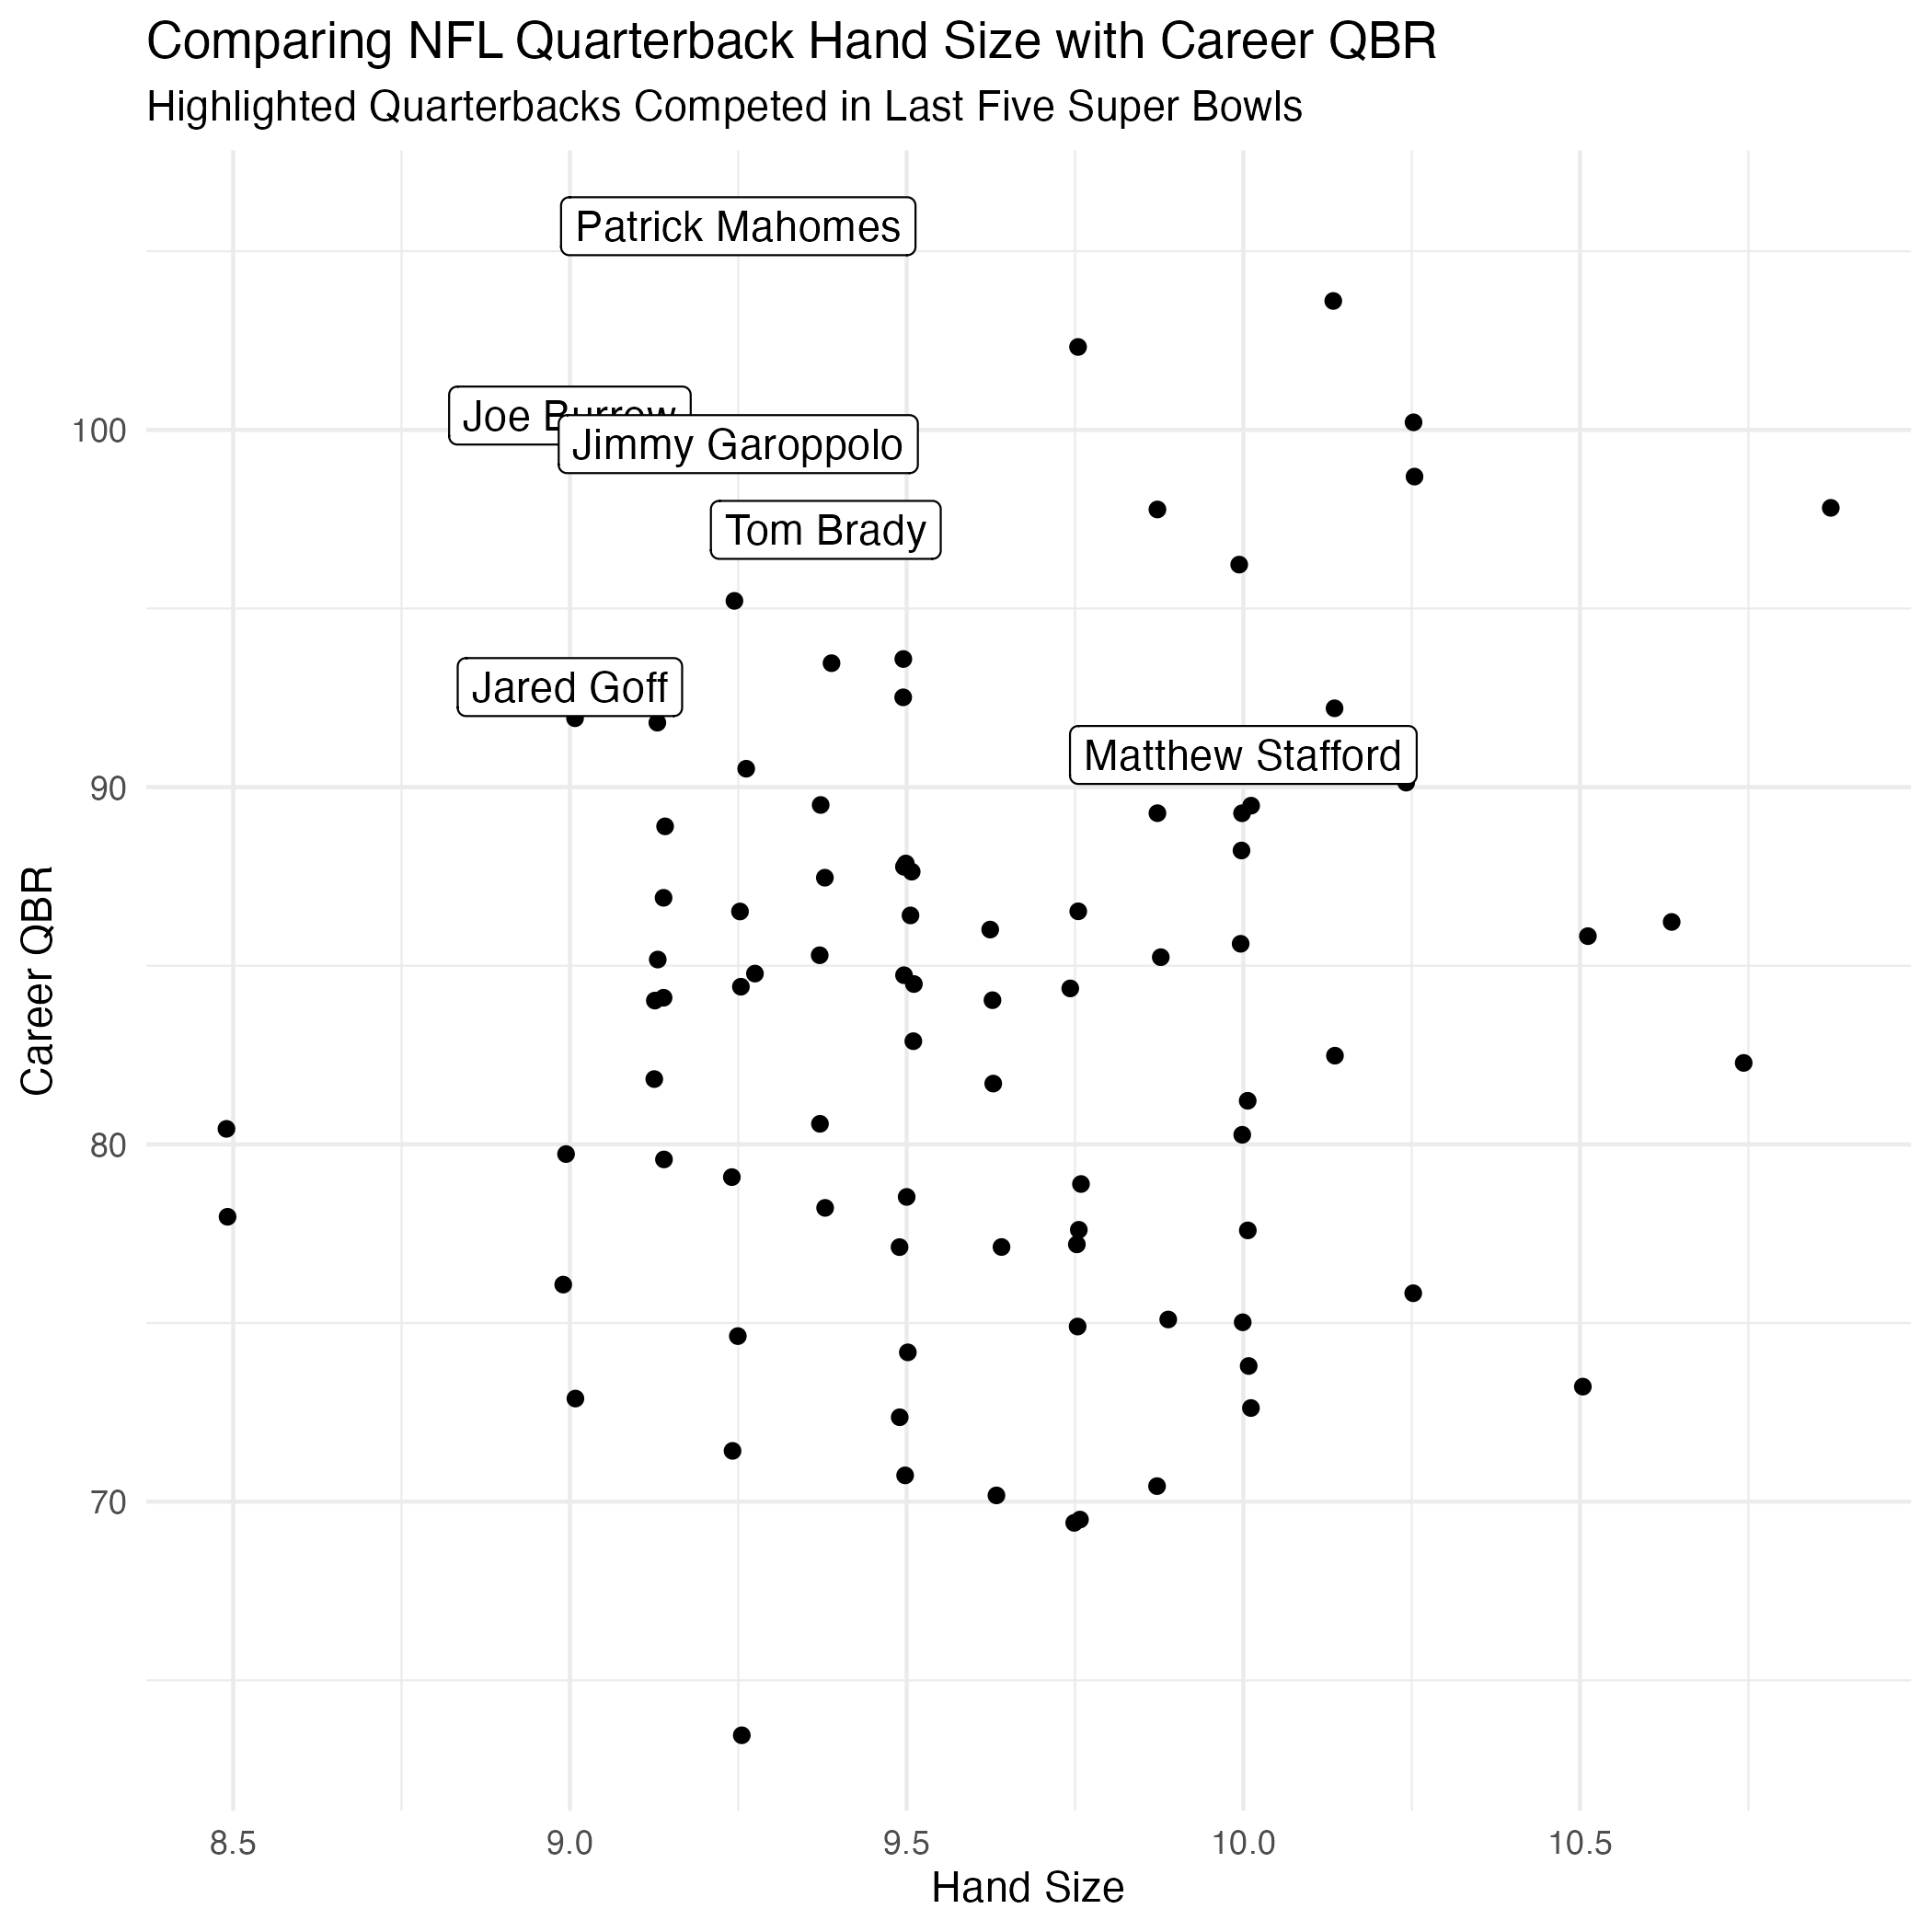
\includegraphics{PS6a_Jones.png}
    \caption{In the first visualization, I created a scatterplot to look and see if there is any relationship between hand size and career performance -- I highlighted the names of quarterbacks that recently played in the superbowl. }
    \label{fig:my_label}
\end{figure}

\begin{figure}
    \centering
    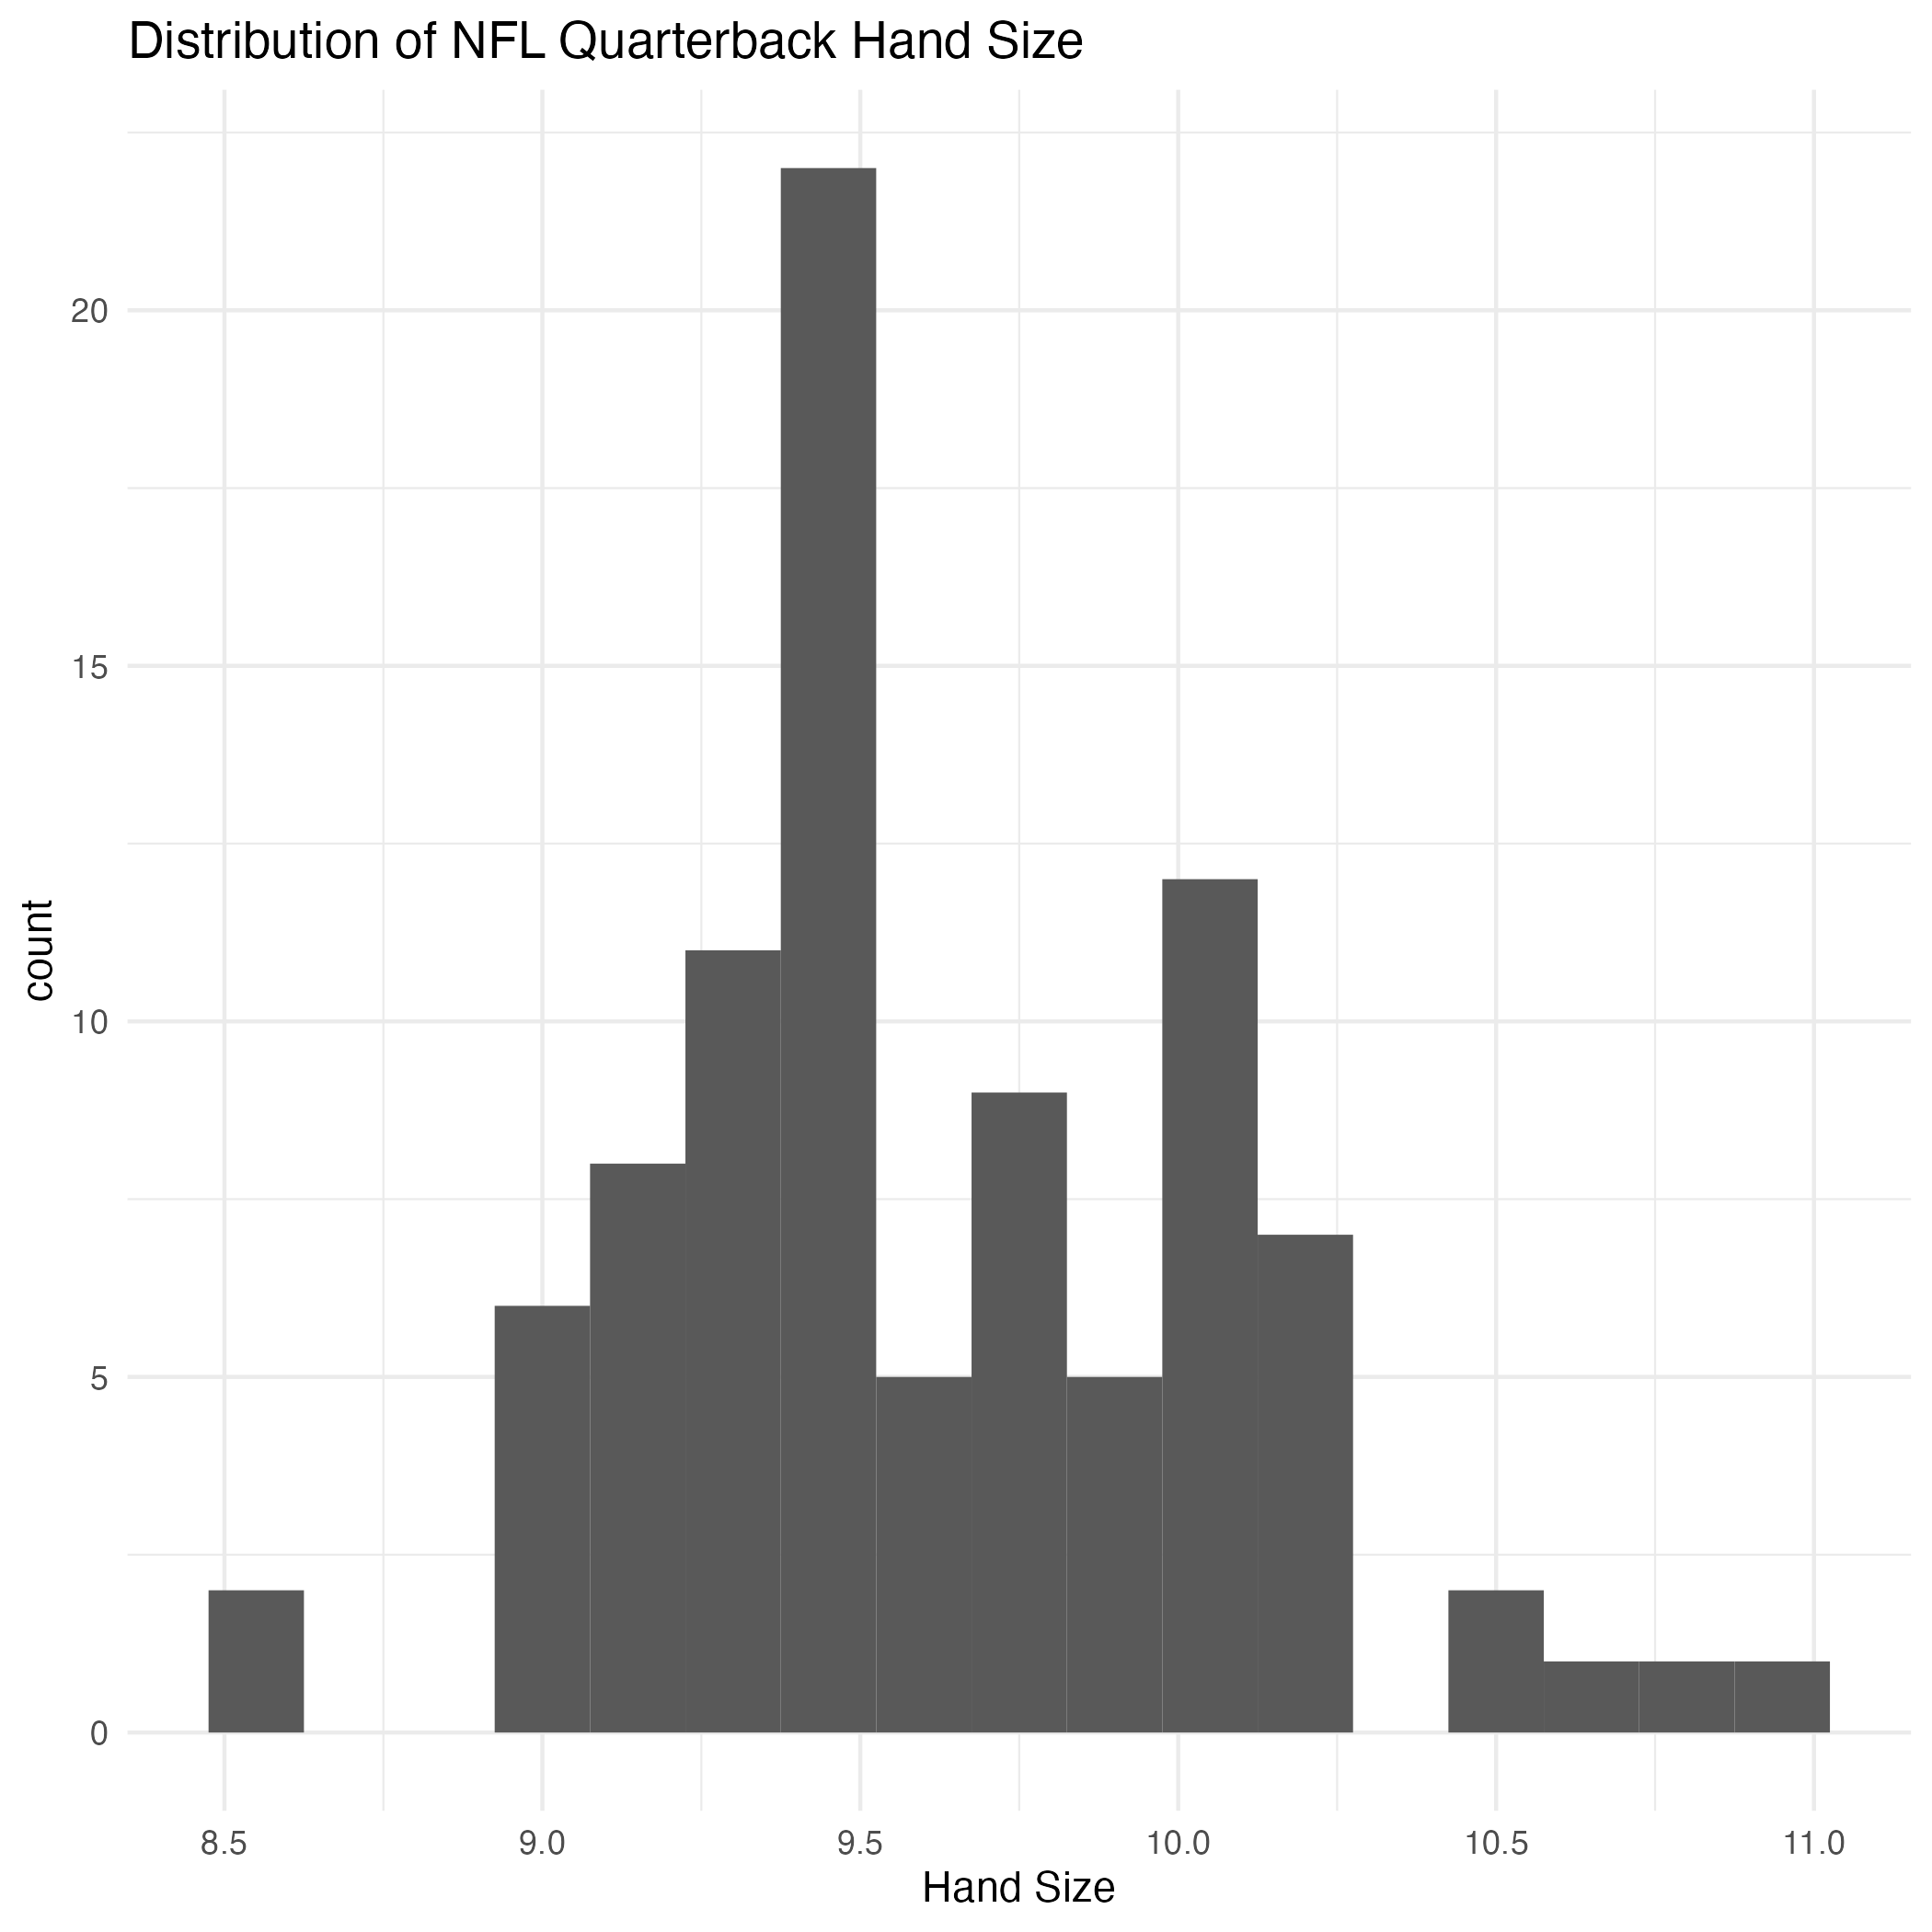
\includegraphics{PS6b_Jones.png}
    \caption{In the second plot, I created a histogram to look at and understand the distribution of hand sizes in the NFL that have been recorded. As you can see, there are a lot between 9.0 inches and 10.0, with outliers on each side. }
    \label{fig:my_label}
\end{figure}

\begin{figure}
    \centering
    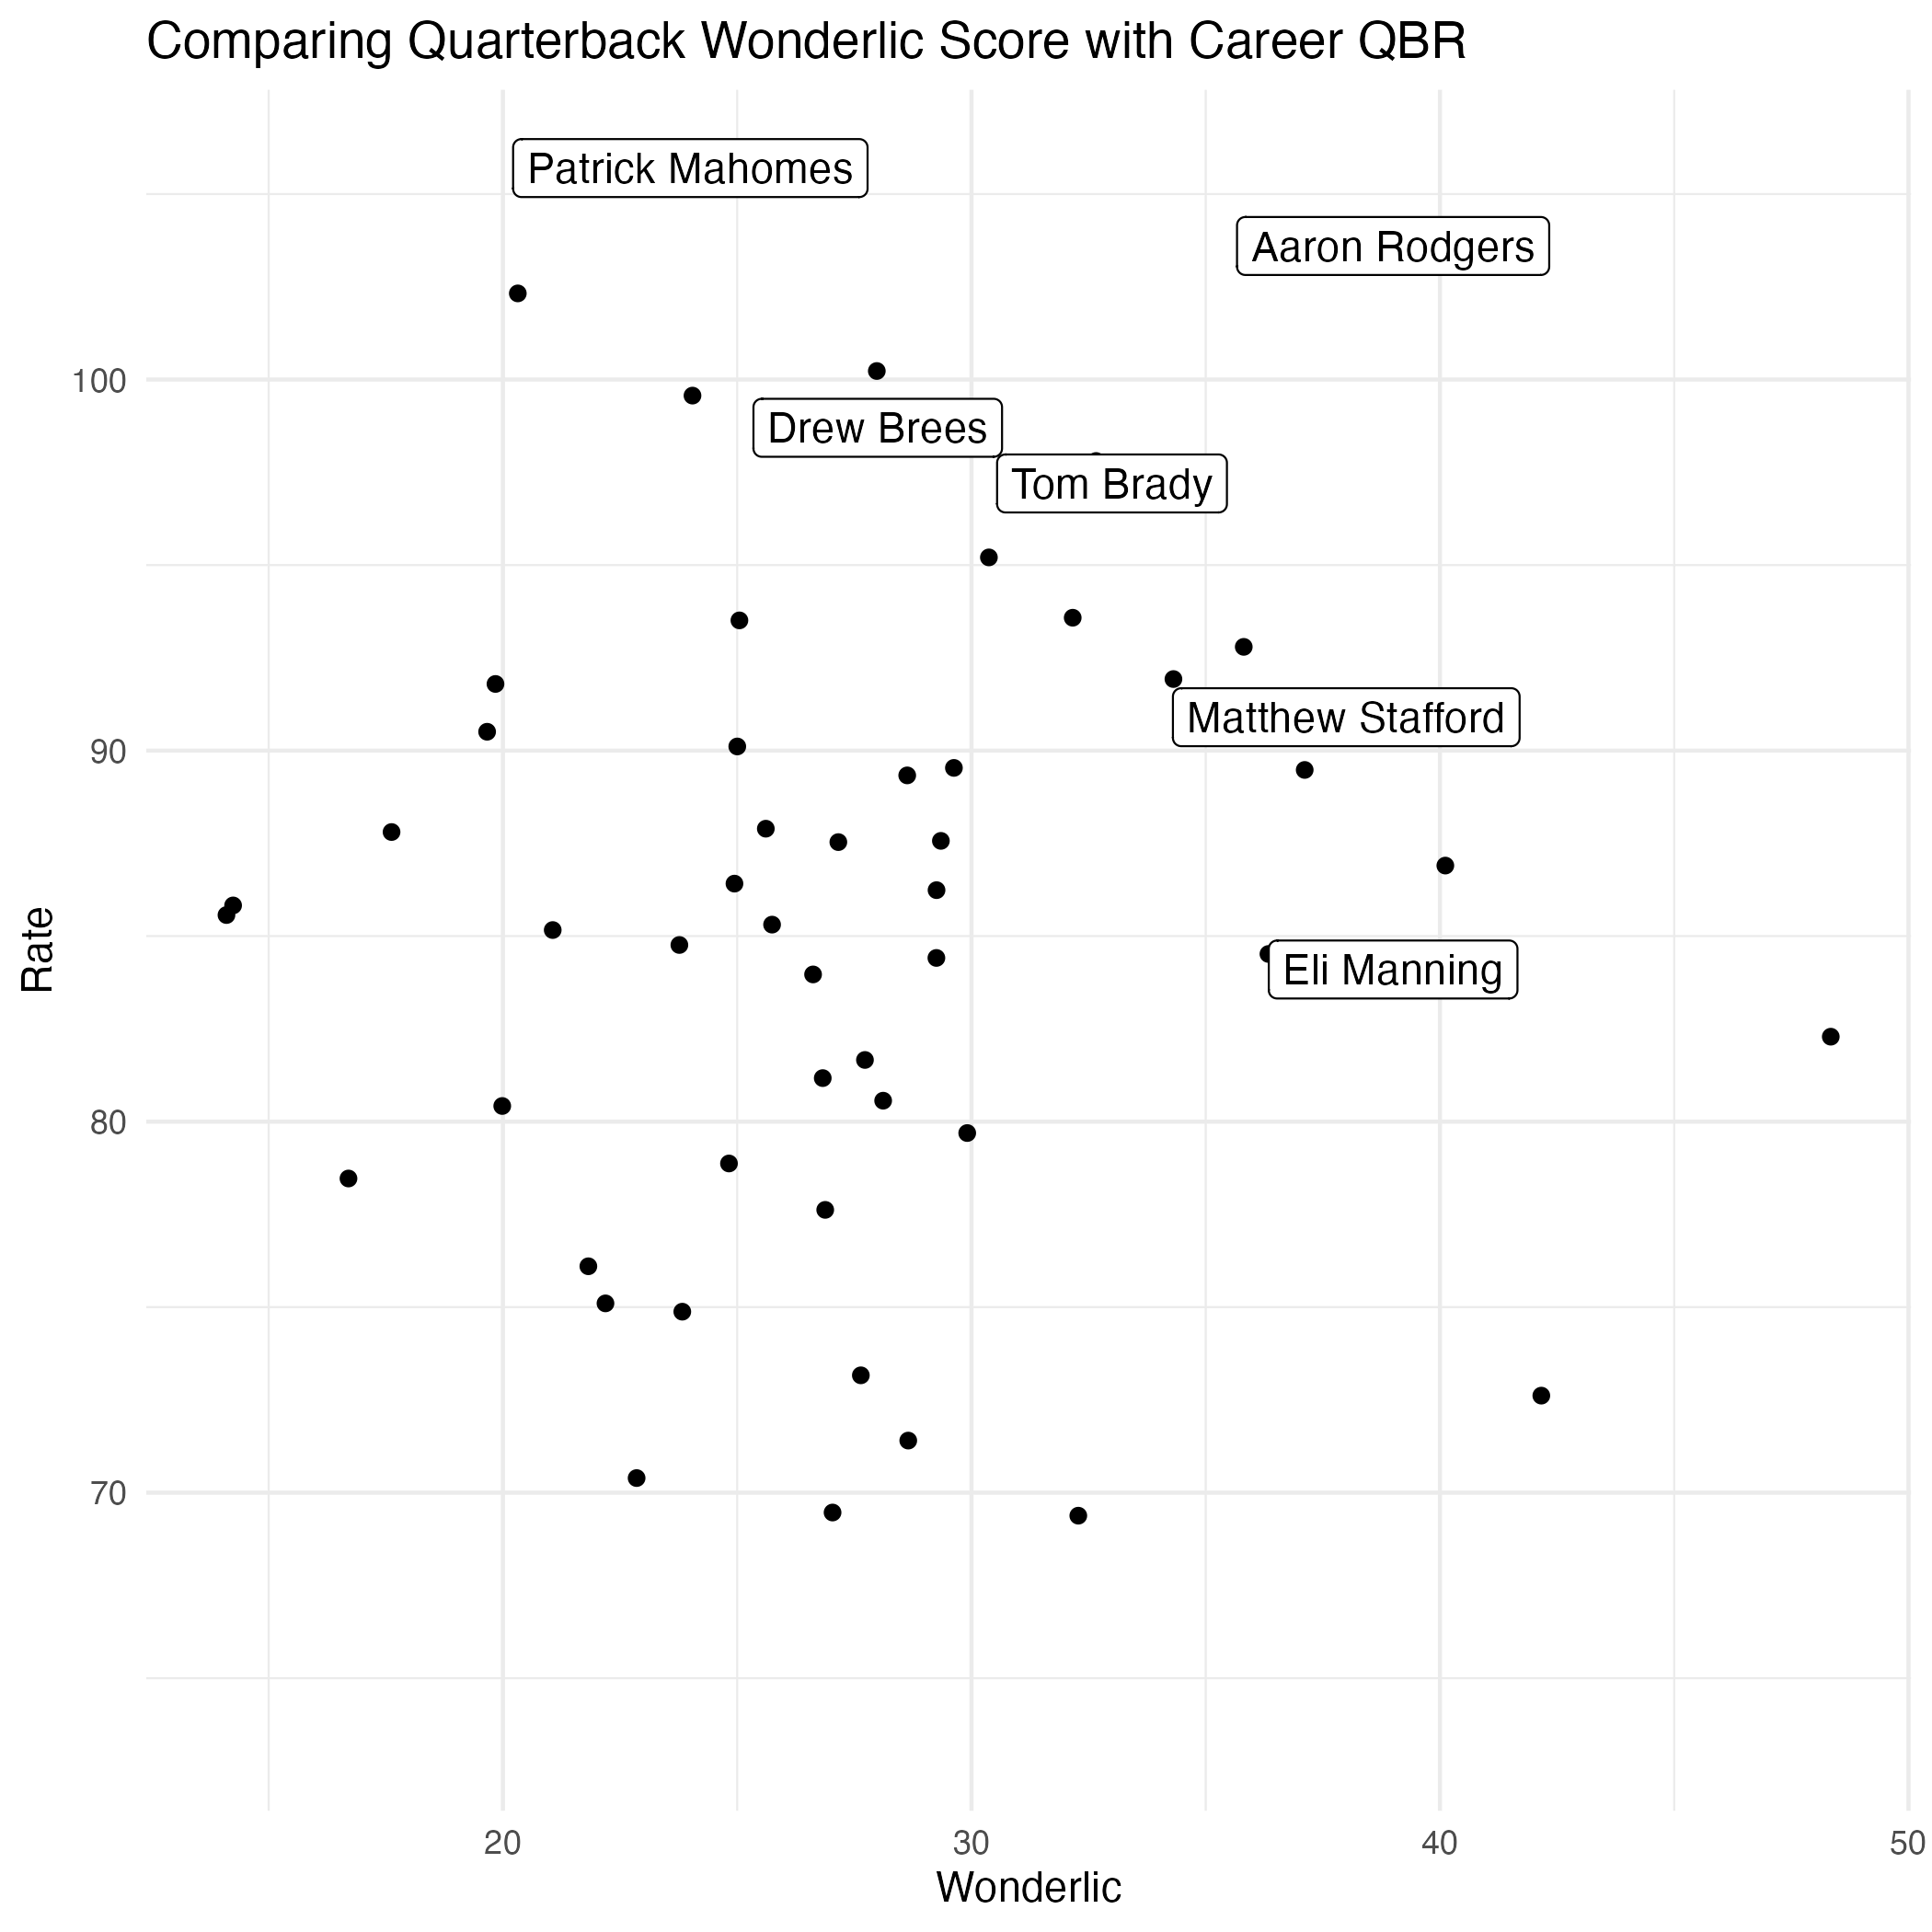
\includegraphics{PS6c_Jones.png}
    \caption{In the third plot, I look at the recorded Wonderlick scores and Career QBR. The Wonderlick test is a general intelligence test given to prospects at the NFL combine. Do higher scoring quarterbacks play better? In recent years many players have refused to take the test, so does it not prove anything well?}
    \label{fig:my_label}
\end{figure}

\end{document}
